\section{Experimental Evaluation}
\label{sec:experiments}

{\bf{Dataset: }} Our model is tested on the PASCAL VOC 2012 segmentation benchmark, which includes 20 foreground object classes and one background class \citep{everingham2014pascal}. The original dataset contains $1,464$, $1,449$, and $1,456$ images for training, validation, and test, respectively. The dataset is augmented by the extra annotations provided by \citep{hariharan2011semantic}, resulting in $10,582$ training images. The performance is measured in terms of pixel intersection-over-union (IOU) averaged across the 21 classes. 

We employ VGG-16 \citep{simonyan2014very} as our DCNN, which is pre-trained on ImageNet \citep{deng2009imagenet}.


{\bf{Weighted loss: }} On the validation set. Without weighted loss: pixel accuracy $90.13\%$, mean class accuracy $73.68\%$, mean Pixel IOU $59.80\%$. With weighted loss: pixel accuracy $66.82\%$, mean class accuracy $88.81\%$, mean pixel IOU $41.77\%$.

{\bf{Incorporate Multi-Scale Features}}
mean PixelIOU $60.25\%$, after crf $64.14\%$.
\begin{figure}[ht]
  \centering
  \begin{tabular}{c c | c c | c c}
      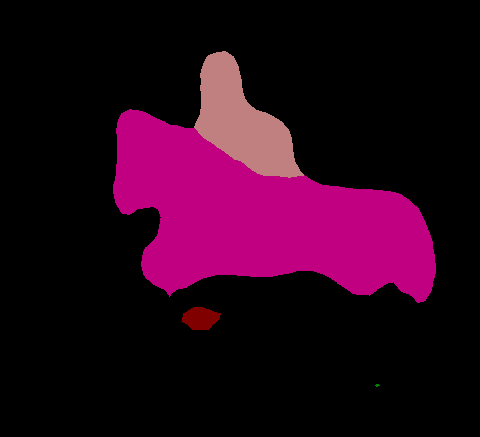
\includegraphics[height=0.12\linewidth]{fig/boundary_refine/vgg128noup_2007_000783.png} &
      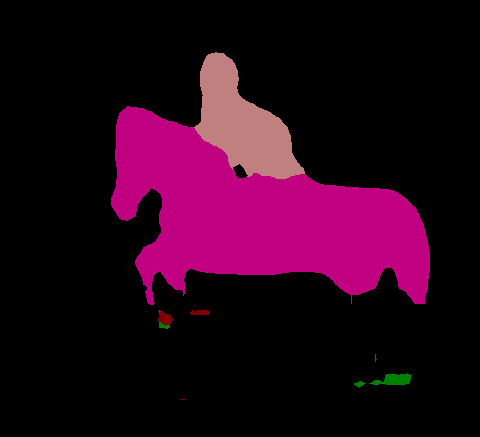
\includegraphics[height=0.12\linewidth]{fig/boundary_refine/vgg128ms_2007_000783.png} &
      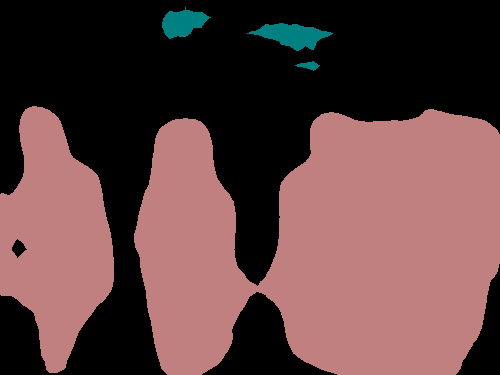
\includegraphics[height=0.12\linewidth]{fig/boundary_refine/vgg128noup_2007_001284.png} &
      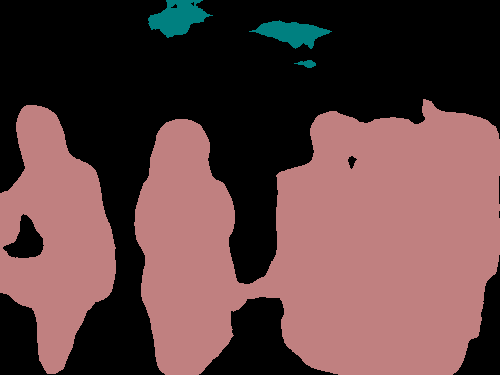
\includegraphics[height=0.12\linewidth]{fig/boundary_refine/vgg128ms_2007_001284.png} &
      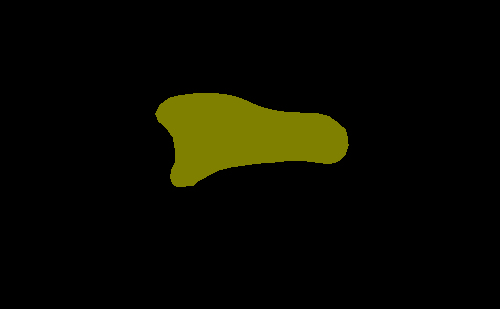
\includegraphics[height=0.12\linewidth]{fig/boundary_refine/vgg128noup_2007_001289.png} &
      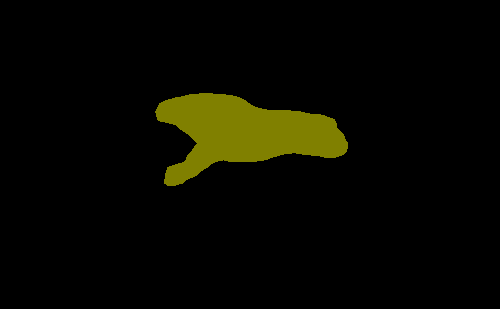
\includegraphics[height=0.12\linewidth]{fig/boundary_refine/vgg128ms_2007_001289.png} \\
      (a) & (b) & (a) & (b) & (a) & (b)
  \end{tabular}
  \label{fig:msBoundary}
  \caption{Incorporating multi-scale features improves the boundary segmentation.}
\end{figure}

{\bf{Incorporate Image-level Feature}} 
mean PixelIOU $59.86\%$, after crf $63.87\%$.

{\bf{Mean Pixel IOU along Object Boundaries: }}
To quantize the improvement of different models, we evaluate the segmention error, defined as (1 - mean IOU), around object boundaries \citep{kohli2009robust, krahenbuhl2011efficient}. Specifically, we take use of the ``void'' label annotated in PASCAL val set, which usually occurs around object boundaries. We compute the mean IOU for those pixels that are located within a narrow band (called trimap) of ``void'' labels. As shown in \figref{fig:IOUBoundary}, adding multi-scale features improve the accuracy slightly. On the other hand, refining the segmentation results by fully connected CRF significantly improve the results around object boundaries. 

\begin{figure}[ht]
  \centering
  \begin{tabular}{c c c | c c}
    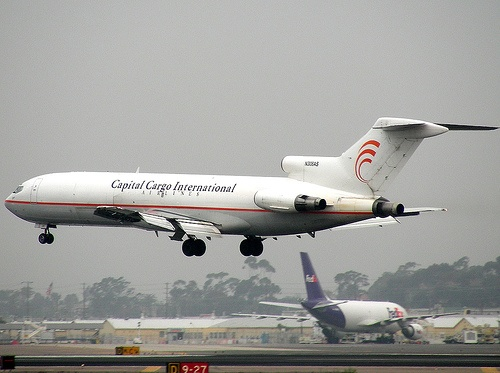
\includegraphics[height=0.12\linewidth]{fig/img/2007_002266.jpg} &
    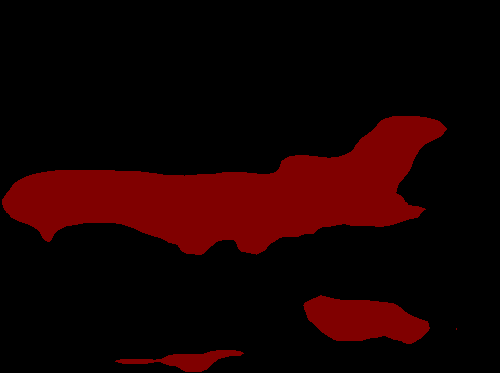
\includegraphics[height=0.12\linewidth]{fig/fcn8s/2007_002266.png} &
    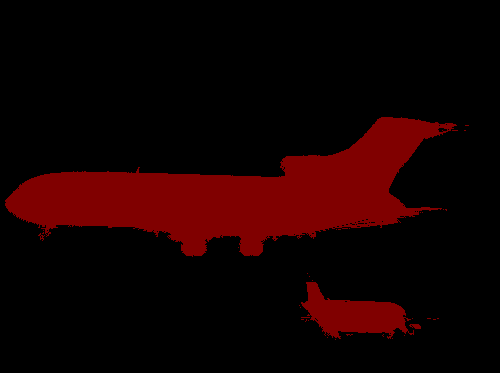
\includegraphics[height=0.12\linewidth]{fig/res_crf/2007_002266.png} &
    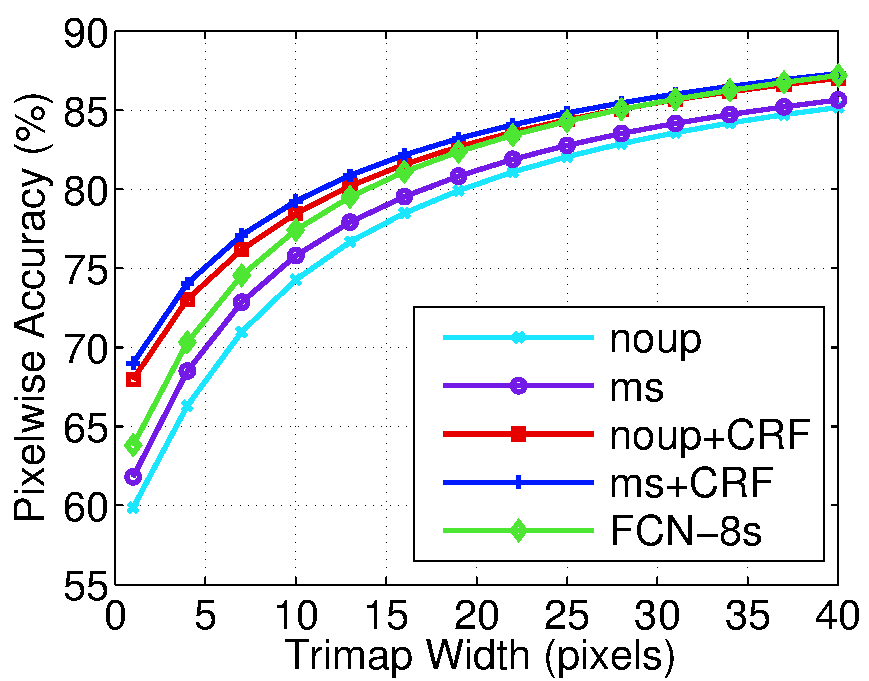
\includegraphics[height=0.12\linewidth]{fig/SegPixelAccWithinTrimap_Berkeley.pdf} &
    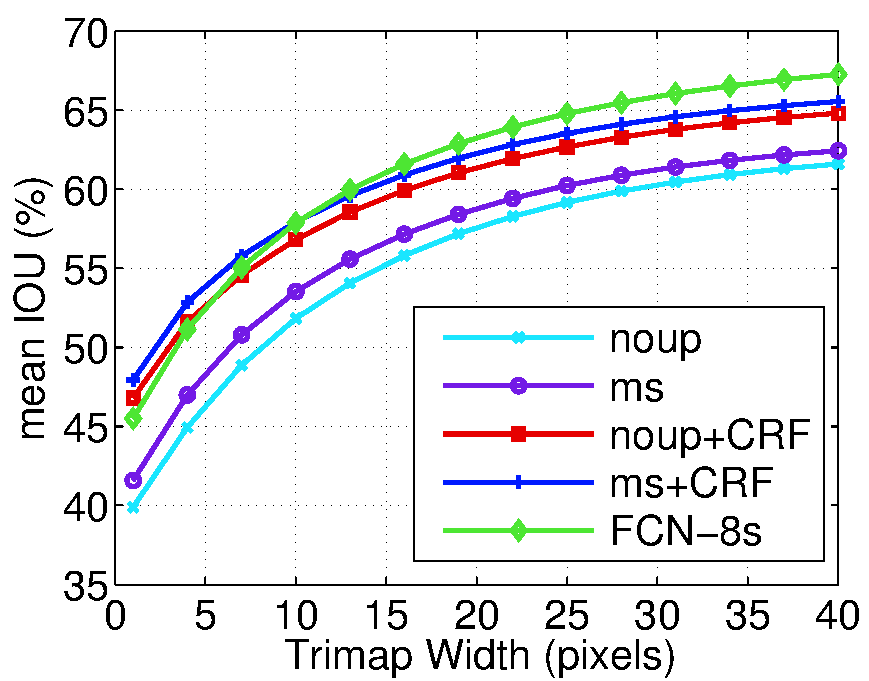
\includegraphics[height=0.12\linewidth]{fig/SegPixelIOUWithinTrimap_Berkeley.pdf} \\
    (a) & (b) & (c) & (d) & (e)
  \end{tabular}
  \caption{(Left) Some comparisons with FCN-8S: (a) image; (b) FCN-8S; (c)
    ms-crf. (d) Segmentation accuracy (pixelwise accuracy) within trimap. (e)
    Segmentation accuracy (mean IOU) within trimap. {\color{red} TODO: change
      legend. HELP: I cannot make them equally spaced....}} 
  \label{fig:IOUBoundary}
\end{figure}

\begin{table*}[t]\scriptsize
\setlength{\tabcolsep}{3pt}
\begin{center}
\begin{tabular}{|c*{20}{|c}||c|}
\hline
bkg &  aero & bike & bird & boat & bottle& bus & car  &  cat & chair& cow &table & dog & horse& mbike& person& plant&sheep& sofa &train & tv   & mean \\
\hline\hline
92.1 & 78.4 & 33.1 & 78.2 & 55.6 & 65.3 & 81.3 & 75.5 & 78.6 & 25.3 & 69.2& 52.7 & 75.2& 69.0 & 79.1 & 77.6 & 54.7 & 78.3 & 45.1 & 73.3 & 56.2 & 66.4\\
\hline
 \end{tabular}
 \caption{Labeling IoU (\%) on the PASCAL VOC 2012 test set
   training on the trainval.}
 \label{tab:voc2012}
 \end{center}
\end{table*}


\begin{figure}[!htbp]
  \centering
  %\vspace{-1.cm}
  \scalebox{0.82} {
  \begin{tabular}{c c c | c c c}
    %\addtolength{\tabcolsep}{-6.5pt}
    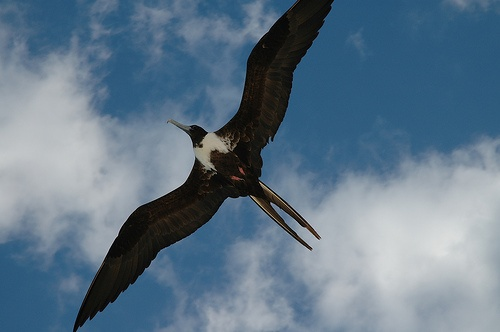
\includegraphics[height=0.12\linewidth]{fig/img/2007_002094.jpg} &
    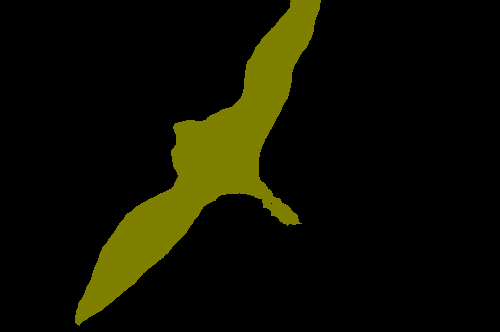
\includegraphics[height=0.12\linewidth]{fig/res_none/2007_002094.png} &
    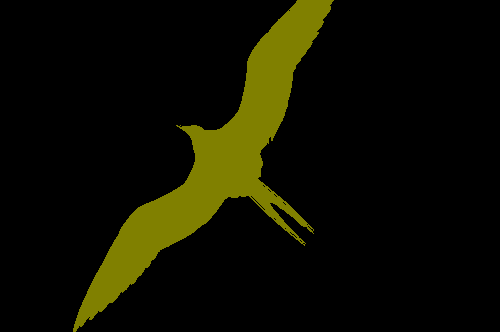
\includegraphics[height=0.12\linewidth]{fig/res_crf/2007_002094.png} &
    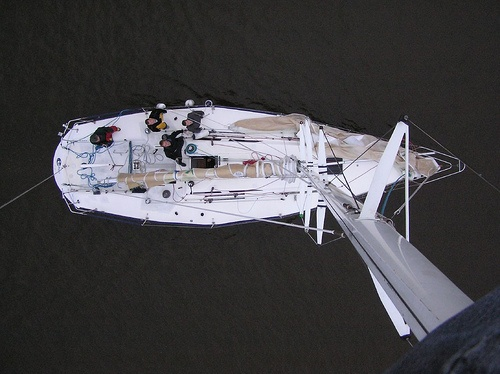
\includegraphics[height=0.12\linewidth]{fig/img/2007_002719.jpg} &
    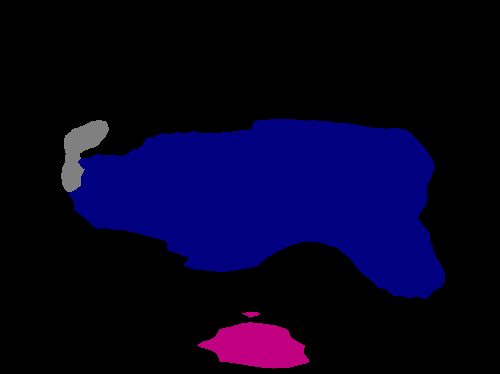
\includegraphics[height=0.12\linewidth]{fig/res_none/2007_002719.png} &
    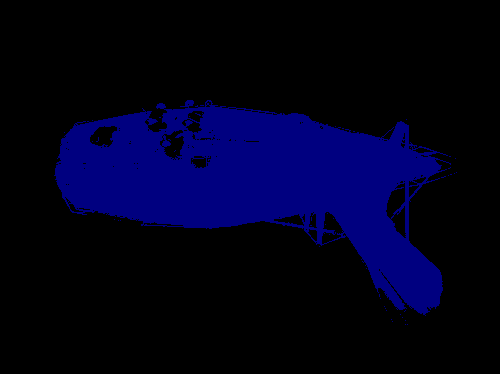
\includegraphics[height=0.12\linewidth]{fig/res_crf/2007_002719.png} \\
    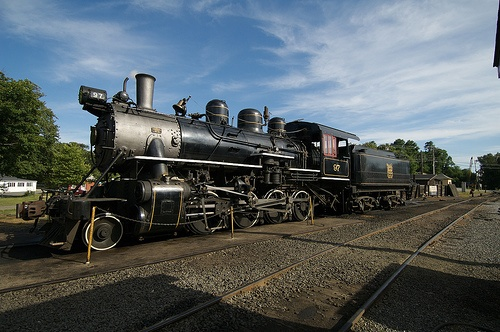
\includegraphics[height=0.12\linewidth]{fig/img/2007_003957.jpg} &
    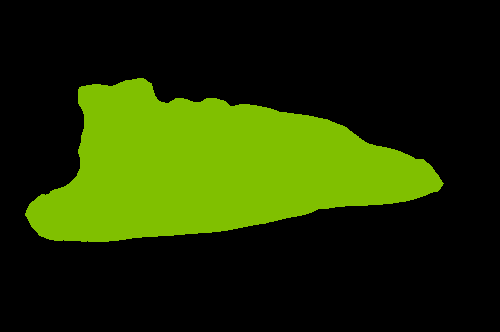
\includegraphics[height=0.12\linewidth]{fig/res_none/2007_003957.png} &
    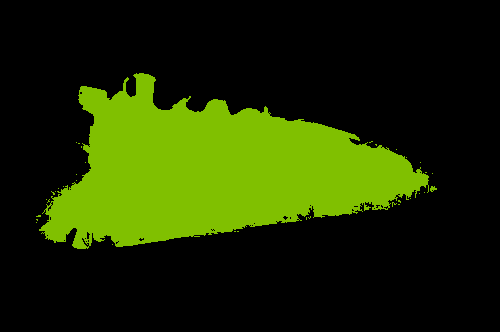
\includegraphics[height=0.12\linewidth]{fig/res_crf/2007_003957.png} &
    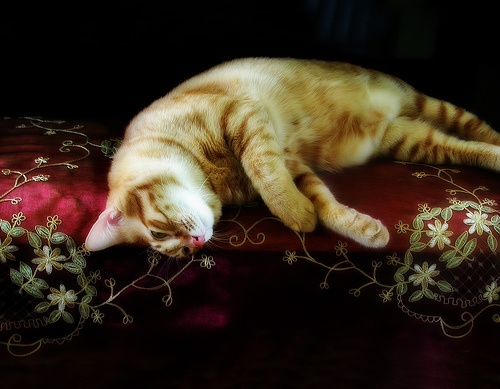
\includegraphics[height=0.12\linewidth]{fig/img/2007_003991.jpg} &
    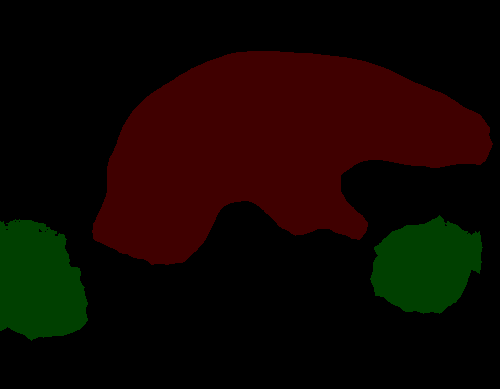
\includegraphics[height=0.12\linewidth]{fig/res_none/2007_003991.png} &
    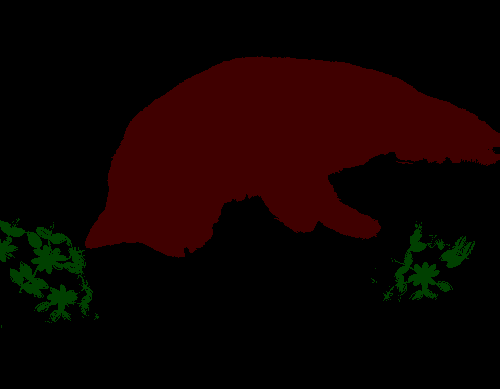
\includegraphics[height=0.12\linewidth]{fig/res_crf/2007_003991.png} \\
    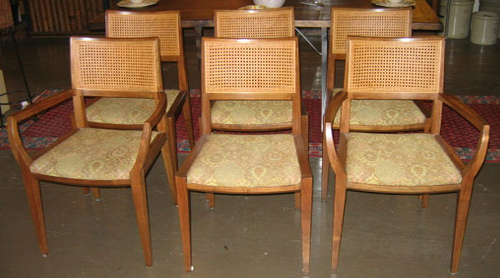
\includegraphics[height=0.10\linewidth]{fig/img/2008_001439.jpg} &
    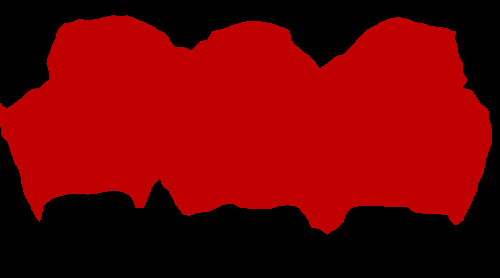
\includegraphics[height=0.10\linewidth]{fig/res_none/2008_001439.png} &
    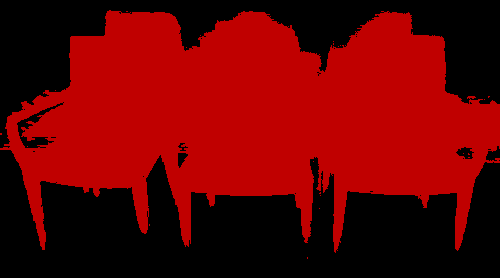
\includegraphics[height=0.10\linewidth]{fig/res_crf/2008_001439.png} &
    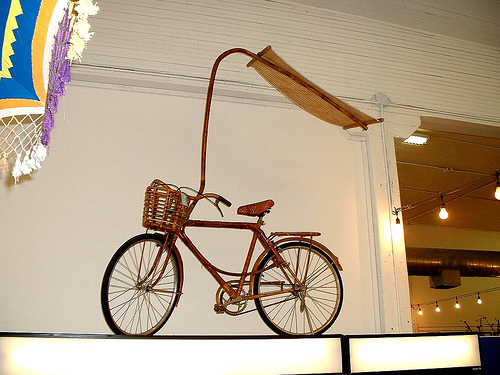
\includegraphics[height=0.12\linewidth]{fig/img/2008_004363.jpg} &
    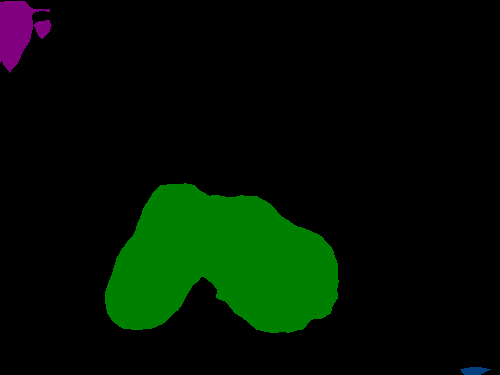
\includegraphics[height=0.12\linewidth]{fig/res_none/2008_004363.png} &
    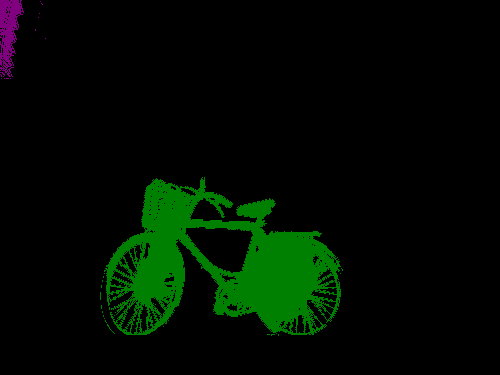
\includegraphics[height=0.12\linewidth]{fig/res_crf/2008_004363.png} \\
    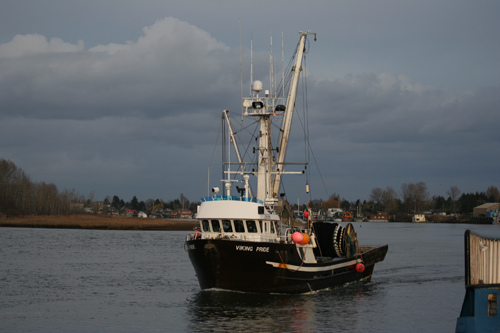
\includegraphics[height=0.12\linewidth]{fig/img/2008_006229.jpg} &
    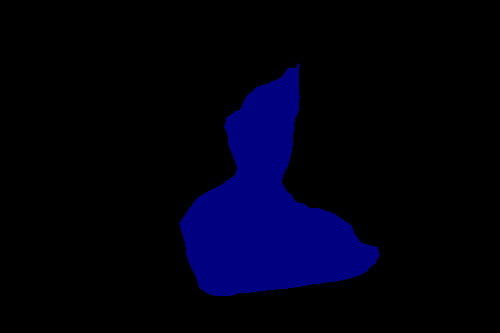
\includegraphics[height=0.12\linewidth]{fig/res_none/2008_006229.png} &
    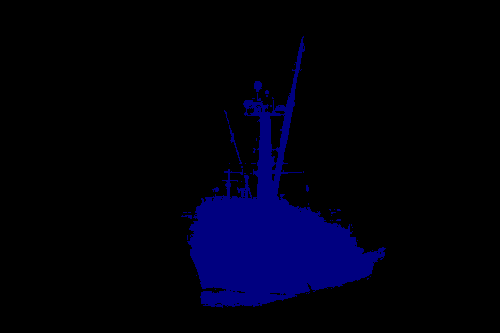
\includegraphics[height=0.12\linewidth]{fig/res_crf/2008_006229.png} &
    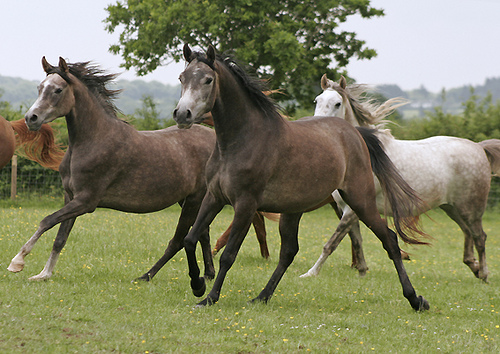
\includegraphics[height=0.12\linewidth]{fig/img/2009_000412.jpg} &
    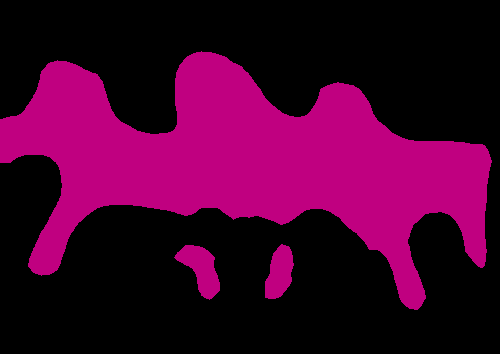
\includegraphics[height=0.12\linewidth]{fig/res_none/2009_000412.png} &
    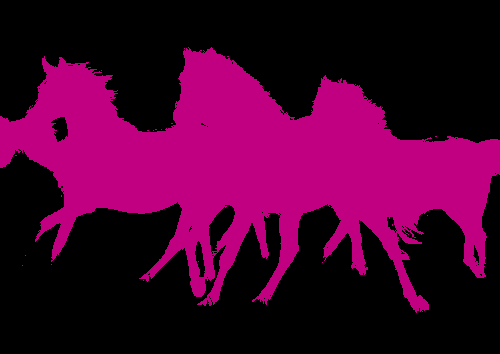
\includegraphics[height=0.12\linewidth]{fig/res_crf/2009_000412.png} \\
    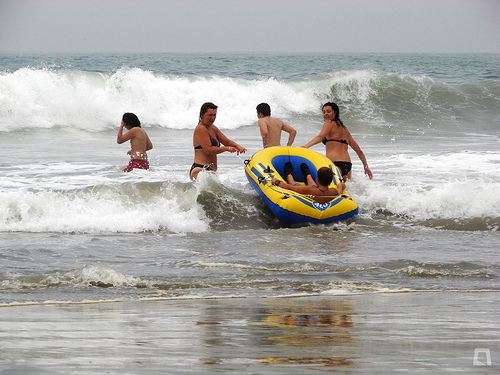
\includegraphics[height=0.12\linewidth]{fig/img/2009_000421.jpg} &
    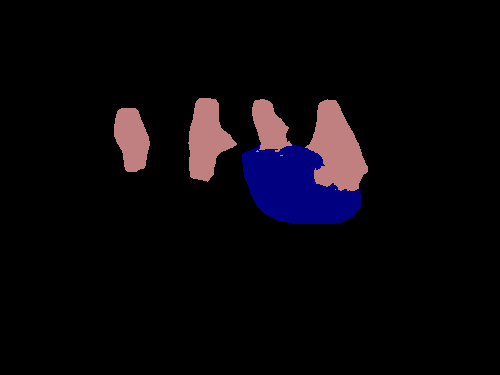
\includegraphics[height=0.12\linewidth]{fig/res_none/2009_000421.png} &
    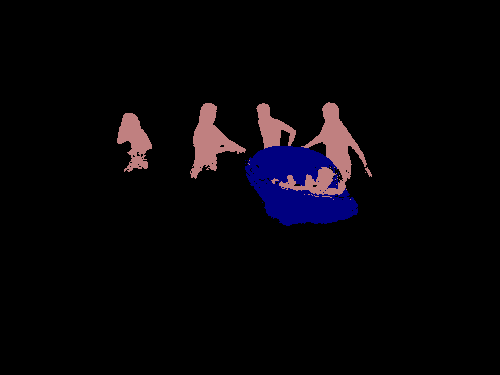
\includegraphics[height=0.12\linewidth]{fig/res_crf/2009_000421.png} &
    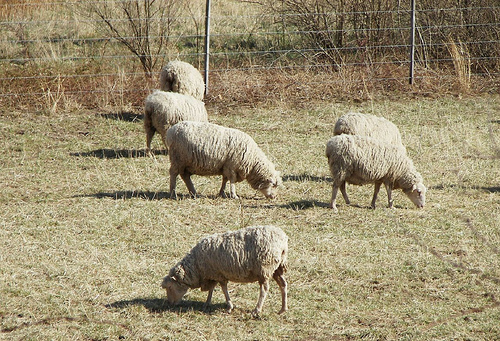
\includegraphics[height=0.12\linewidth]{fig/img/2010_001079.jpg} &
    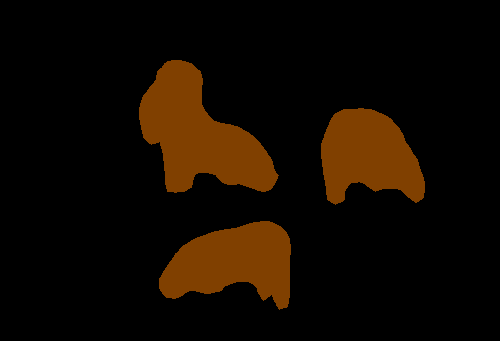
\includegraphics[height=0.12\linewidth]{fig/res_none/2010_001079.png} &
    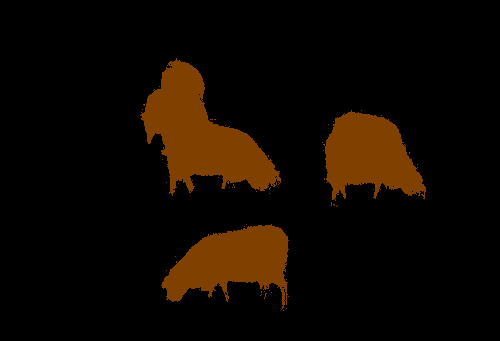
\includegraphics[height=0.12\linewidth]{fig/res_crf/2010_001079.png} \\
    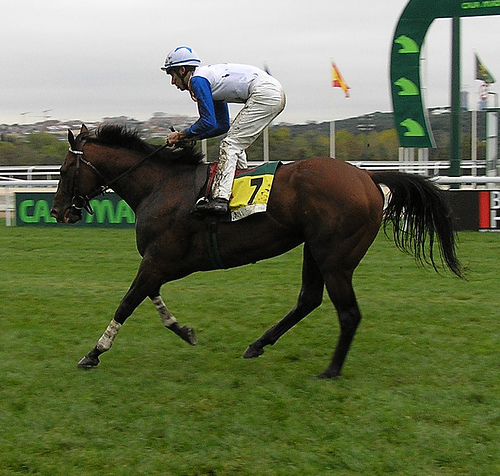
\includegraphics[height=0.12\linewidth]{fig/img/2010_000038.jpg} &
    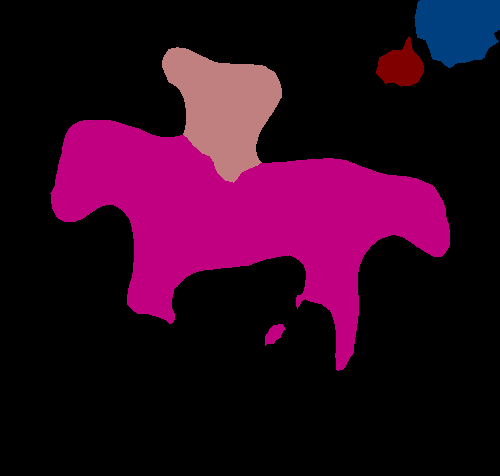
\includegraphics[height=0.12\linewidth]{fig/res_none/2010_000038.png} &
    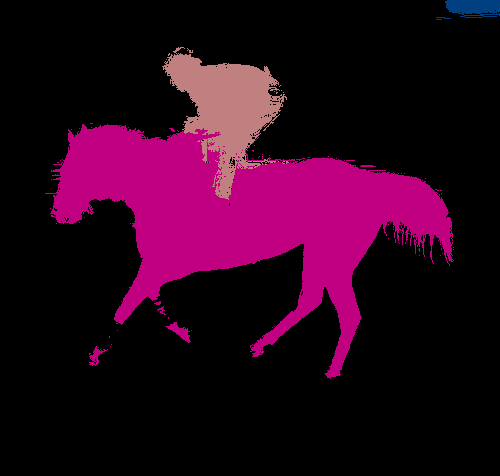
\includegraphics[height=0.12\linewidth]{fig/res_crf/2010_000038.png} &
    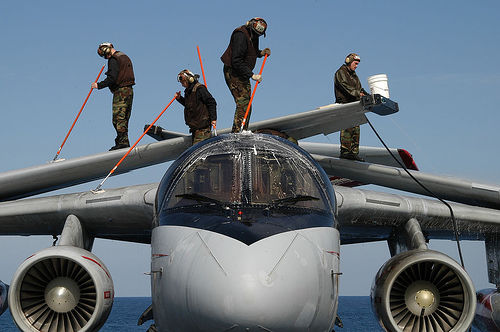
\includegraphics[height=0.12\linewidth]{fig/img/2010_001024.jpg} &
    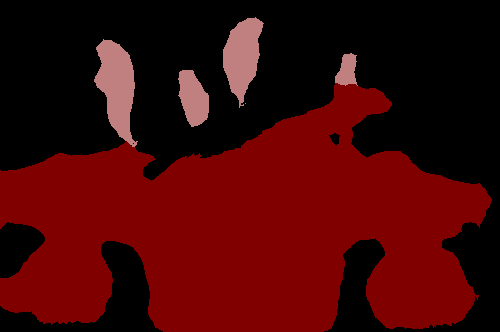
\includegraphics[height=0.12\linewidth]{fig/res_none/2010_001024.png} &
    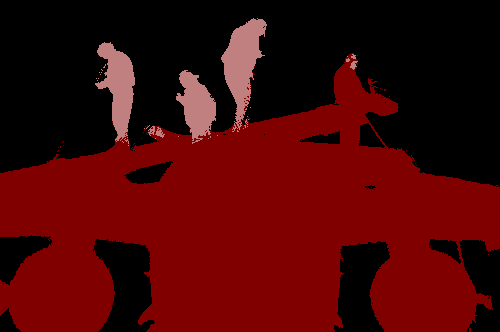
\includegraphics[height=0.12\linewidth]{fig/res_crf/2010_001024.png} \\
    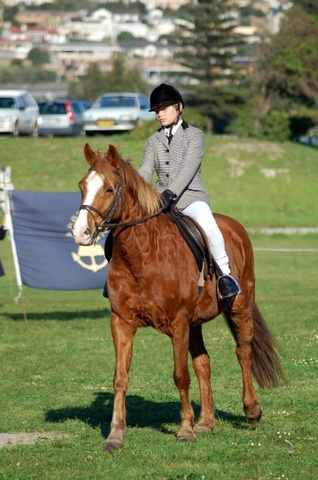
\includegraphics[height=0.24\linewidth]{fig/img/2007_005331.jpg} &
    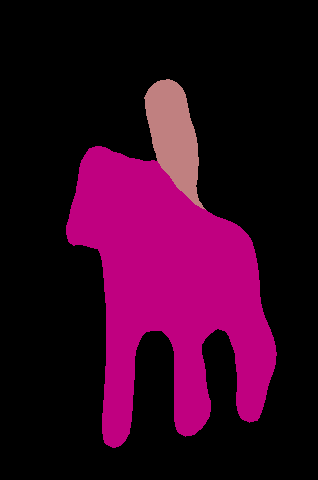
\includegraphics[height=0.24\linewidth]{fig/res_none/2007_005331.png} &
    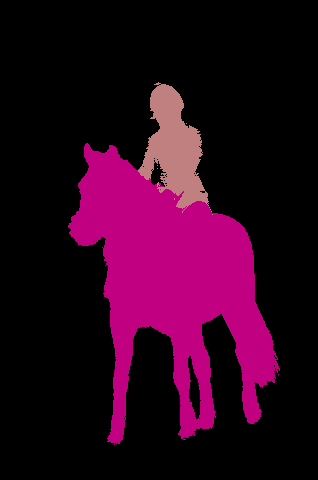
\includegraphics[height=0.24\linewidth]{fig/res_crf/2007_005331.png} &
    \includegraphics[height=0.24\linewidth]{fig/img/2008_004654.jpg} &
    \includegraphics[height=0.24\linewidth]{fig/res_none/2008_004654.png} &
    \includegraphics[height=0.24\linewidth]{fig/res_crf/2008_004654.png} \\
    \includegraphics[height=0.24\linewidth]{fig/img/2007_000129.jpg} &
    \includegraphics[height=0.24\linewidth]{fig/res_none/2007_000129.png} &
    \includegraphics[height=0.24\linewidth]{fig/res_crf/2007_000129.png} &
    \includegraphics[height=0.24\linewidth]{fig/img/2007_002619.jpg} &
    \includegraphics[height=0.24\linewidth]{fig/res_none/2007_002619.png} &
    \includegraphics[height=0.24\linewidth]{fig/res_crf/2007_002619.png} \\
    \includegraphics[height=0.12\linewidth]{fig/img/2007_002852.jpg} &
    \includegraphics[height=0.12\linewidth]{fig/res_none/2007_002852.png} &
    \includegraphics[height=0.12\linewidth]{fig/res_crf/2007_002852.png} &
    \includegraphics[height=0.12\linewidth]{fig/img/2010_001069.jpg} &
    \includegraphics[height=0.12\linewidth]{fig/res_none/2010_001069.png} &
    \includegraphics[height=0.12\linewidth]{fig/res_crf/2010_001069.png} \\
    \hline
    \hline
    \includegraphics[height=0.12\linewidth]{fig/img/2007_000491.jpg} &
    \includegraphics[height=0.12\linewidth]{fig/res_none/2007_000491.png} &
    \includegraphics[height=0.12\linewidth]{fig/res_crf/2007_000491.png} &
    \includegraphics[height=0.12\linewidth]{fig/img/2007_000529.jpg} &
    \includegraphics[height=0.12\linewidth]{fig/res_none/2007_000529.png} &
    \includegraphics[height=0.12\linewidth]{fig/res_crf/2007_000529.png} \\
    \includegraphics[height=0.12\linewidth]{fig/img/2007_000559.jpg} &
    \includegraphics[height=0.12\linewidth]{fig/res_none/2007_000559.png} &
    \includegraphics[height=0.12\linewidth]{fig/res_crf/2007_000559.png} &
    \includegraphics[height=0.12\linewidth]{fig/img/2007_000663.jpg} &
    \includegraphics[height=0.12\linewidth]{fig/res_none/2007_000663.png} &
    \includegraphics[height=0.12\linewidth]{fig/res_crf/2007_000663.png} \\    
  \end{tabular}
  }
  %\vspace{-0.3cm}
  \caption{Visualization results on VOC 2012 val. For each row, we show image, segmentation result by CNN, and refined segmentation result by Fully Connected CRF. We show our failure modes in teh last two rows.} 
  \label{fig:ValResults}
\end{figure}
